\begin{figure}[H]
\centering
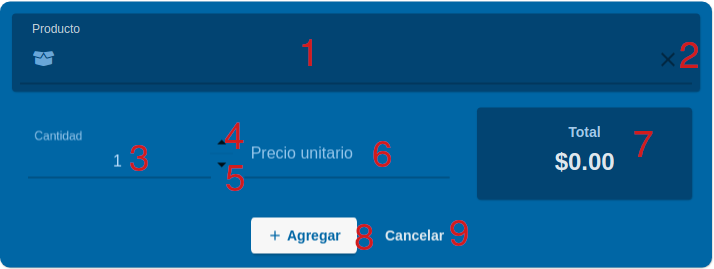
\includegraphics[width=\textwidth,height=\textheight,keepaspectratio]{Escenarios/AD-05-00}
\caption{Escenario - AD-05-00}
\label{fig:AD-05-00}
\end{figure}
Este es el escenario que permite a los usuarios crear o modificar lineas de presupuesto y lineas de venta. En el campo \textbf{AD-05-01} el usuario indicará el producto con el cual se está creando o bien el nuevo producto en caso de estar modificando. El botón \textbf{AD-05-02} permite eliminar la selección del campo \textbf{AD-05-01}. El campo \textbf{AD-05-03} indica la cantidad de producto elegido, con un click en los botones \textbf{AD-05-04} y \textbf{AD-05-05} se incrementa y se decrementa una unidad del campo \textbf{AD-05-03} respectivamente. El campo\textbf{AD-05-06}, se automcompletará con el precio unitario del producto y podrá ser editado por el usuario en caso de contar con los permisos. El campo \textbf{AD-05-07} mostrará el total que será calculado como el producto por el precio unitario por la cantidad.
Un click en el botón \textbf{AD-05-08} creará o modificará la linea de presupuesto o de venta y navegará al escenario \textbf{AD-04-00} o \textbf{AD-11-00} según corresponda, mientras que un click en el botón \textbf{AD-05-09} descartará todos los cambios realizados y navegará al escenario \textbf{AD-04-00} o \textbf{AD-11-00} según corresponda.
\clearpage
